All participants we interviewed worked as a part of a team, we asked everyone to describe their team in order to gain insight in the circumstances surrounding the retrospective.  One of the teams, team Echo, was large with ten people working on several different products at the same time. The team was then divided in the subject where members worked on one or more products, this led to a small amount of infighting and divisions. The retrospectives were also affected as not everyone had the same experiences or problems. This led to time being wasted for team members as issues beyond their scope were discussed in plenum. In team Alfa and team Foxtrot this was not mentioned as a problem. 

Team Charlie was a small team of four developers, where all were highly experienced, with especially two of the developers holding very senior positions within the company. The two senior developers were described as especially strong personalities. The team was described as very eager to learn and always searching for ways and ideas that could be used to improve the team. The strong personalities influenced the retrospectives in that sometimes the junior developers would agree without arguing strongly for their own ideas or suggestions. Another interview participant from team Delta also described his team as very eager and they considered the retrospective meetings the most important process during development. 



\section{Feedback Session: Team Discussion}
After performing our content analysis, we visited the team to present our analysis results as well as receive feedback from the team. In this section and its following sub-sections we'll present the results from this session. We will start with going through the feedback on the key numbers, before we continue on the categories and trends and finally take anything else that came up during the session. 

\subsection{Feedback: Categories and Trends}
In this section we will present the thoughts of the team as well as their reactions on the results of the content analysis. We will start with the nature of the actions and then continue on context, decision making, organizational learning and development phase and finally we will go through the collaboration categories and trends. 

\subsection{Other Feedback From the Feedback Session}
Several other things were mentioned by the team during the feedback session. 

\section{Feedback Session 2: Interview with SCRUM Master}
The interview lasted for almost 1 hour, and was recorded and transcribed. At the start of the interview we did a short recap of the presentation. During this recap the interviewee expressed satisfaction with the analysis, and agreed with the constructed framework for analysis. The interview revolved around three main subjects that were discussed, team dynamics, organizational learning and retrospectives.

\section{Feedback Session 3: Team Leader}
\label{second-feedback-results}
The start of the third feedback session revolved around discussing event analysis, where the amount of actions were plotted next to events like staff change or secretary changes. The session revealed two major changes after our first analysis, as well as a process change. The first major change that was mentioned was that the focus of the retrospective had become more positive, with participants making sure to bring up positive issues. This change was considered an improvement by the team leader. A second change was a different attitude in the team towards the unresolved retrospective actions. The previous attitude was to think of the list of unresolved actions as a great mass that just grew, with little appreciation for the large number of actions and improvements were accomplished. The team leader expressed that this had led to a more positive environment. The team also planned to include retrospective actions in a maintenance day that was held at regular day, in order to make sure that resources were delegated to solving the actions. 

\subsection{Effect of outside perspective}


\section{Interview Results}
In this section, and its following subsections, we will present our results from the semi-structured interviews. We will present the results in relation to the different themes discussed during the interview: ``General'', ``Organizational Learning'', ``Team Dynamics''and ``Anything Else''. We will not present every statement made by all the interviewees, but focus on the unique results that came out of the interviews. 

It was also mentioned that only the actions doesn't necessary reflect the complete retrospective meeting. Good things are usually not created to actions as may other things be. 




















\subsection{Retrospectives Techniques}
There are a lot of ways to perform retrospective. Around the table discussion, story-telling, weather-forecast and many more are examples of ways to conduct retrospectives. We will briefly describe two commonly used technique called KJ-session and timeline. Other techniques can be found by reading Derby and Larsen's book\cite{Larsen2006}: \textit{``Agile Retrospectives: Making Good Teams Great!''}, accessing the web page Retromat.org\cite{retromat2015} or reading our own literature review on the agile retrospective\cite{Dolvik2014}. 

\subsubsection{KJ-session}
KJ-sessions are a commonly used brainstorming technique where each participant write issues on post-it notes after the participants are done the post-it notes are grouped and discussed in the group. Dingsøyr, Moe and Nytrø\cite{Moe2001} provides an example of they conducted a KJ-session and the end-result of a KJ-session can be seen in \autoref{figure:kj-session}: 

\begin{quote}
We used a technique named after a Japanese ethnologist, Jiro
Kawakita - called the KJ-method. For each of these sessions,
we give the participants a set of post-it notes, and ask them to
write one issue on each. We usually hand out between three and
five notes per person, depending on the number of participants.
After some minutes, we ask one of them to attach one note to a
whiteboard and say why this issue was important. Then the next
person would present a note and so on until all the notes are on
the whiteboard. The notes are then grouped, and each group is
given a new name. 
\end{quote}

\begin{figure}[!h]
	\centering
	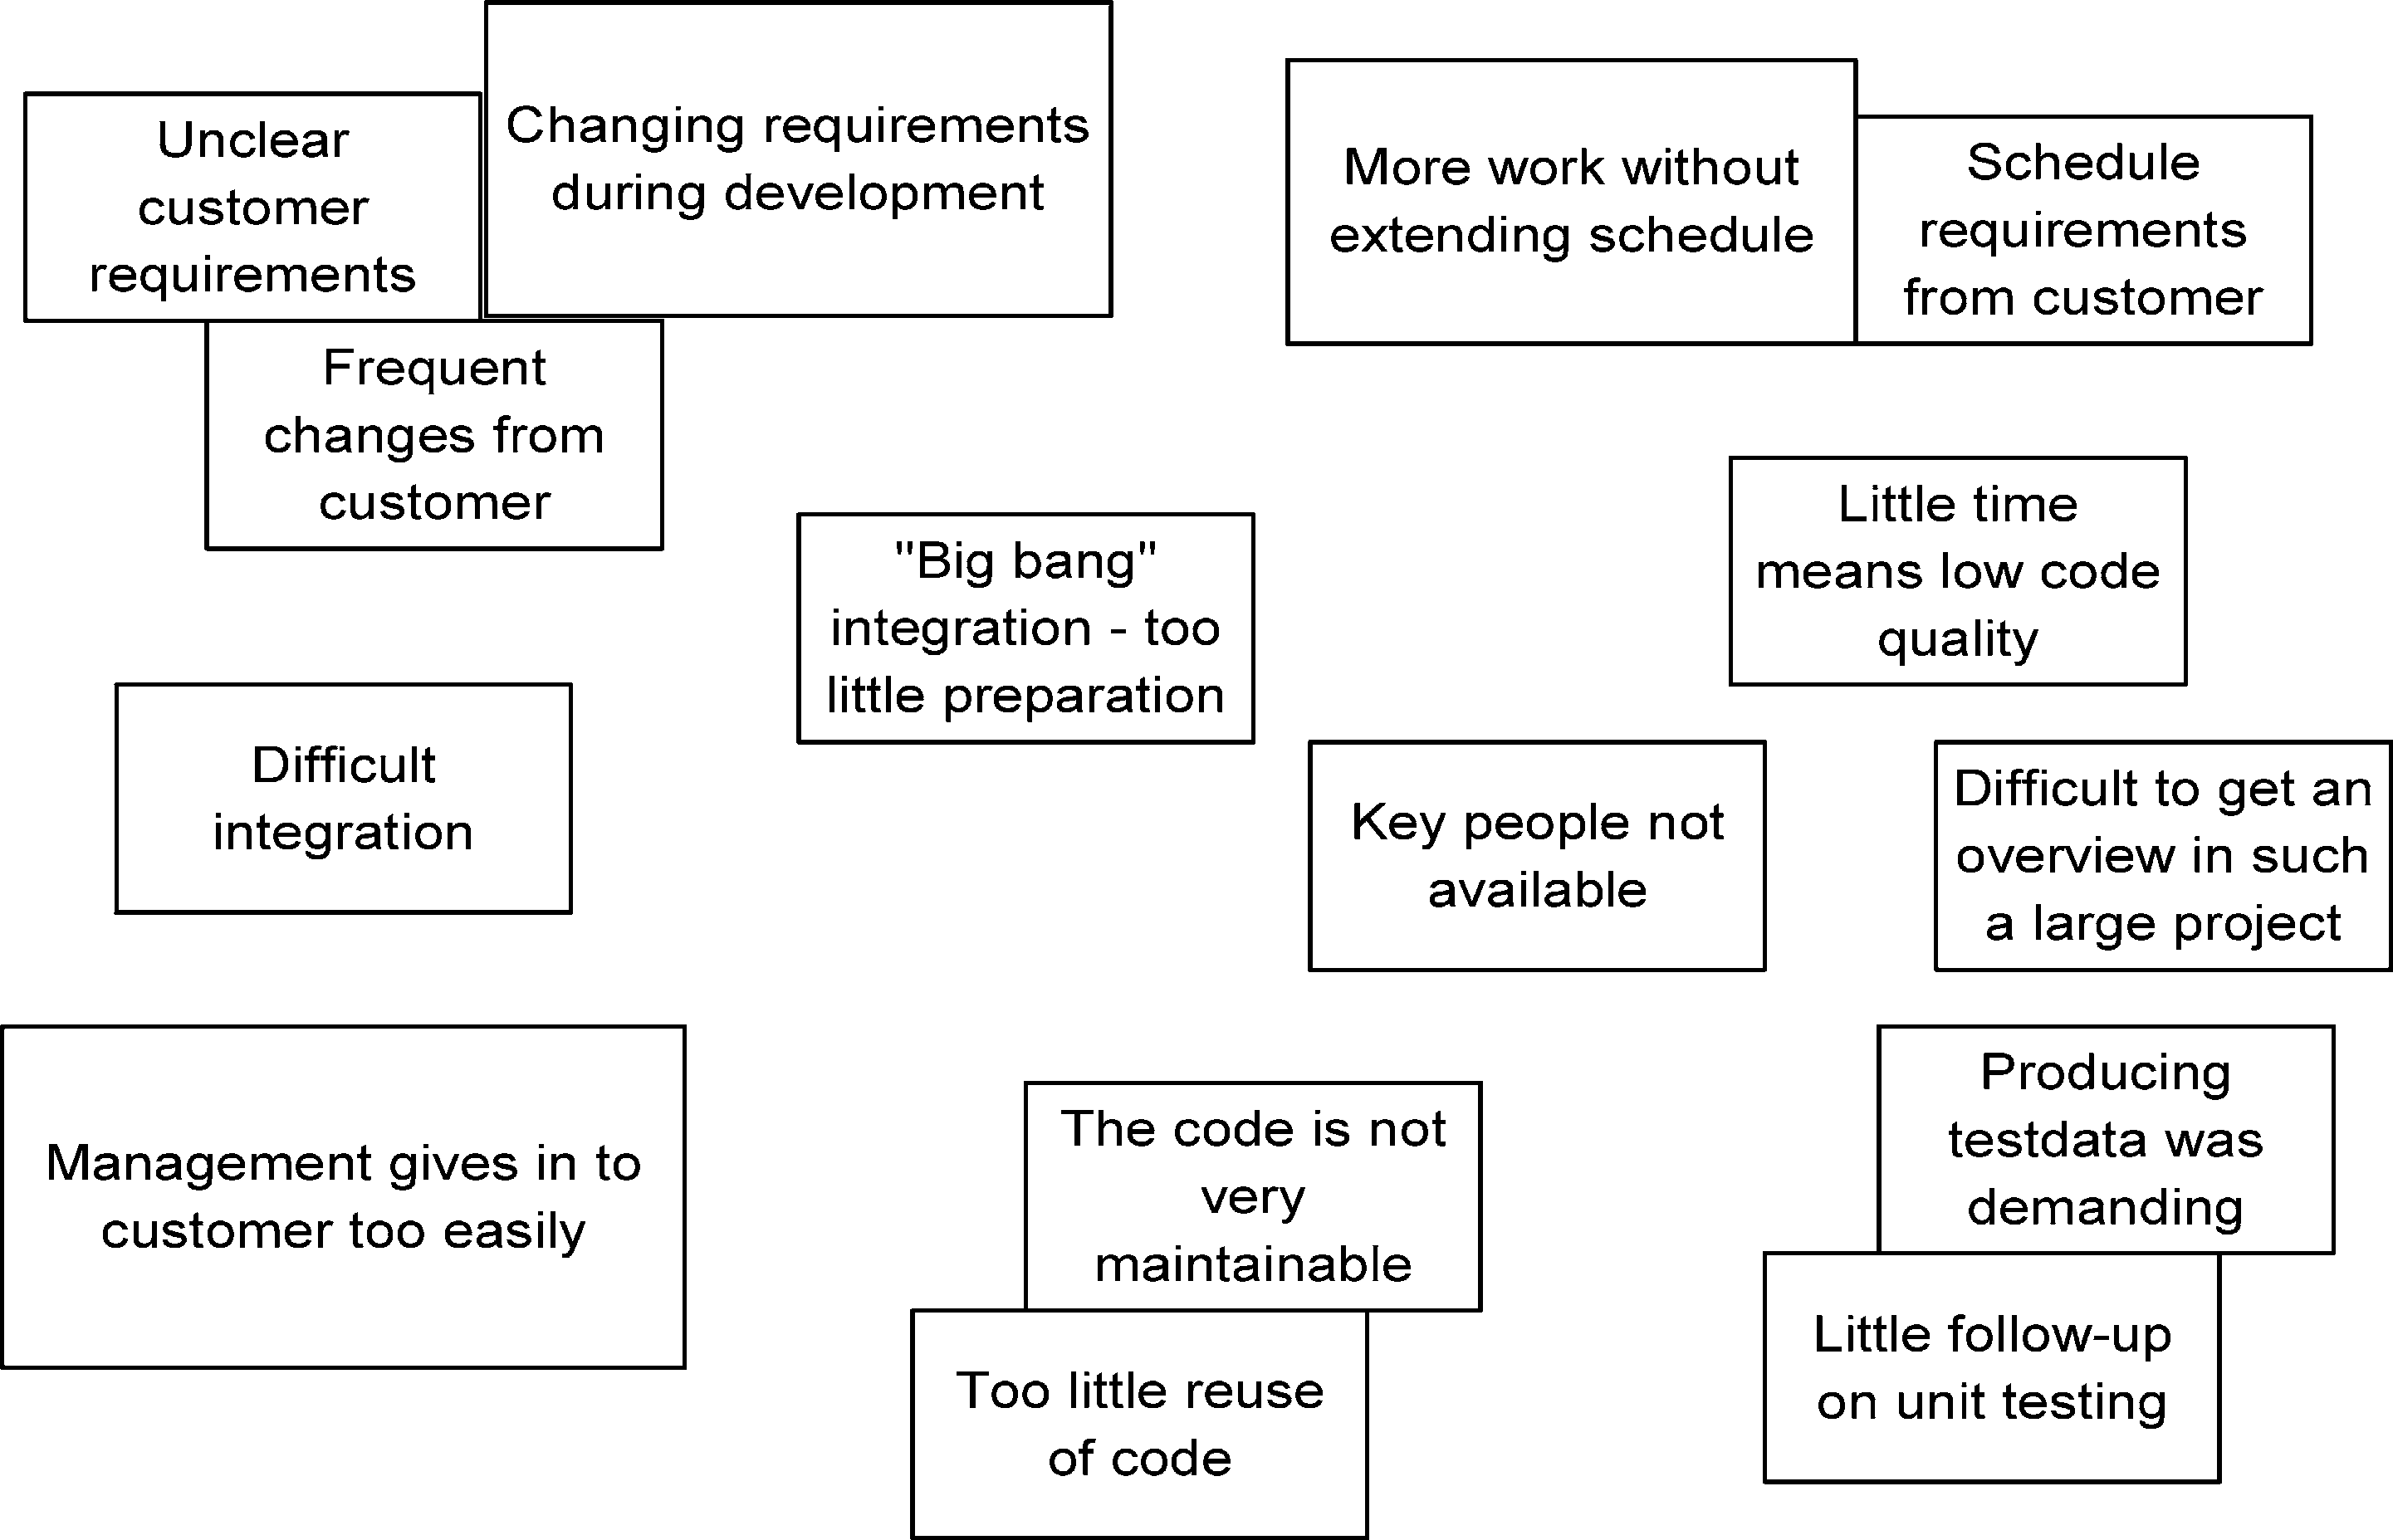
\includegraphics[width=\textwidth, keepaspectratio]{figures/KJ-session.png}
	\caption{KJ-session end result, provided by Dingsøyr\cite{Dingsoyr2004}}
	\label{figure:kj-session}
\end{figure}

\subsubsection{Timeline}
Timeline is an activity that lets the participants create a timeline over the last learning event and reflect on the event during the creation. Derby and Larsen\cite{Larsen2006} suggests that the participants should be divided into multiple groups. Each member in the group should then be handed markers and post-it notes and then write their own issues from the learning event down. Derby and Larsen suggests color-coding the post-it notes relating them to feelings, events, functions or themes. When all the participants are done writing they should together create a timeline with the post-it notes. After the timeline is done the group should analyze the timeline, looking for interesting patterns and opportunities for future improvements. An example timeline is shown in \autoref{figure:timeline}.

\begin{figure}[!h]
	\centering
	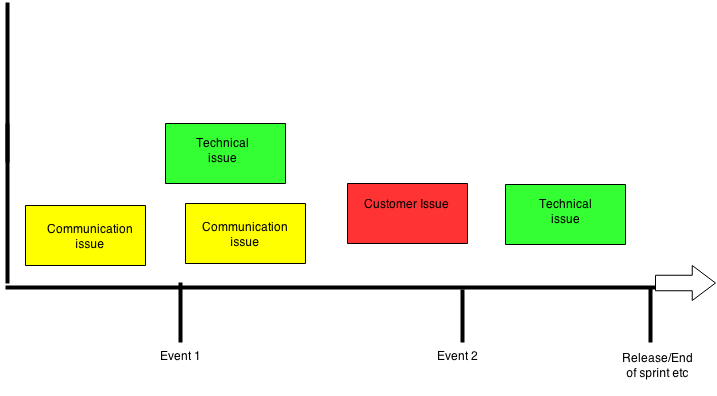
\includegraphics[width=\textwidth, keepaspectratio]{figures/Timeline-Example.png}
	\caption{Timeline illustration}
	\label{figure:timeline}
\end{figure}

There also exists a variation of timeline called; Evidence-Based Timelines, which is described by Bjarnason and Regnell\cite{Bjarnason2012}. The difference from normal timeline retropsective is that the data is collected through available systems before the retrospective. The idea is to counter bias from the participants where memory lacks and thus rather use data collected from available system during the time-period in question. A graphic example is presented by Bjarnason and Regnell and shown in \autoref{figure:e-b-timeline}. 

\begin{figure}[!h]
	\centering
	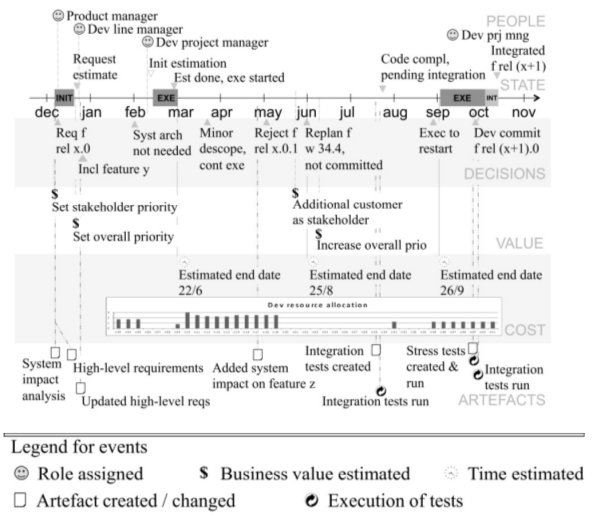
\includegraphics[width=\textwidth, keepaspectratio]{figures/eb-timeline.png}
	\caption{Evidence-based timeline illustration, presented by Bjarnason and Regnell\cite{Bjarnason2012}}
	\label{figure:e-b-timeline}
\end{figure}

\section{Content Analysis Results}
From the retrospective reports we obtained several interesting results. We will go through each of them below starting with some key numbers and then move on to the results of the content analysis. Then we identify some trends observed while performing the content analysis. 